%\documentclass[letterpaper,fontsize=20pt]{scrartcl}
\usepackage{tikz}
\usepackage{tikzpagenodes}
\usepackage{scrlayer-scrpage}
\usepackage[final]{pdfpages}
%\usepackage{lipsum}
\usepackage{fontspec}
\usepackage[english]{babel}
\usepackage{blindtext}
\usepackage[absolute,overlay]{textpos}

\definecolor{myblue}{RGB}{13, 43, 109}

\definecolor{myblue2}{RGB}{53, 166, 217}

\newcommand{\blueborder}{\tikz[remember picture,overlay] 
    \draw [myblue,line width=22mm]
    (current page.south west)
    rectangle
    (current page.north east)
    ;}


%\usepackage{lipsum}
%\begin{document}
\renewcommand\maketitle{
\begin{titlepage}
\chead[\blueborder]{\blueborder} % for page borders
    \null\vfil
\blueborder
\linespread{2} 
\begin{textblock*}{15cm}(3.5cm,6cm) % {block width} (coords) 
\noindent
\textcolor{myblue}{\textbf{ \huge OpenACC Programming \newline and Best Practices Guide}}
%\textcolor{myblue}{\textbf{\fontspec{QTHelvetCnd} \huge OpenACC Programming \newline and Best Practices Guide}}

\noindent
%\textcolor{myblue2}{\fontspec{Liberation Sans Narrow} November 2020}
\textcolor{myblue2}{\@date}
\end{textblock*}

\begin{textblock*}{19.408cm}(0.36cm,13cm)
\begin{figure}
 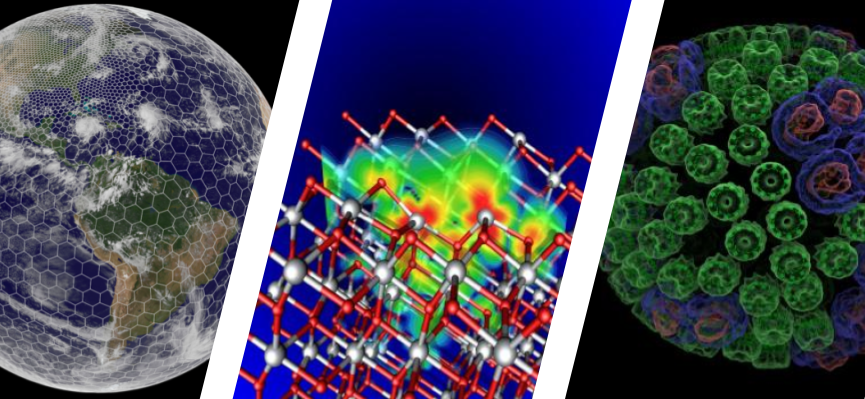
\includegraphics[width=\textwidth]{cover-page/app_images.png}
\end{figure}
\end{textblock*}

\begin{textblock*}{10.7cm}(8.7cm,22.3cm)
\begin{figure}[hb!]
 
\includegraphics[width=\textwidth]{cover-page/logo.png}
\end{figure}
\end{textblock*}

\begin{textblock*}{10.7cm}(1.8cm,26.3cm)
\textcolor{myblue}{ \tiny © 2022 openacc-standard.org. All Rights Reserved.}
%\textcolor{myblue}{\fontspec{QTHelvetCnd} \tiny © 2020 openacc-standard.org. All Rights Reserved.}
\end{textblock*}

\pagenumbering{gobble}
%\newpage
%\newpage
%\cleardoublepage
\linespread{1} 
\vfil\null
\end{titlepage}
}

%\end{document}
